\chapter{Introduction}

% What is MS

\section{Motivation}

\subsection[A short introduction to multiple sclerosis]{A Short Introduction to
Multiple Sclerosis}

\Gls{ms} is a chronic and degenerative disease of the \gls{cns} characterized by
the formation of inflammatory and demyelinating lesions. Presumably due to the
breakdown of the blood-brain-barrier, the body's own immune system attacks the
myelin sheaths that act as insulating covers of the axons of neurons. This
disrupts the ability of parts of the nervous system to communicate, and can lead
to the manifestation of a large range of different signs and symptoms. The brain
is a very plastic organ and is often able to compensate for the damage by
forming new neural pathways. In the later stages of the diseases however, the
amount of tissue damage is often to high to be compensated in addition to signs
of axonal loss and neurodegeneration, which leads to the progressive
accumulation of disease.

\begin{figure}[tb]
\centering
\begin{tikzpicture}
\node[] (healthy)
{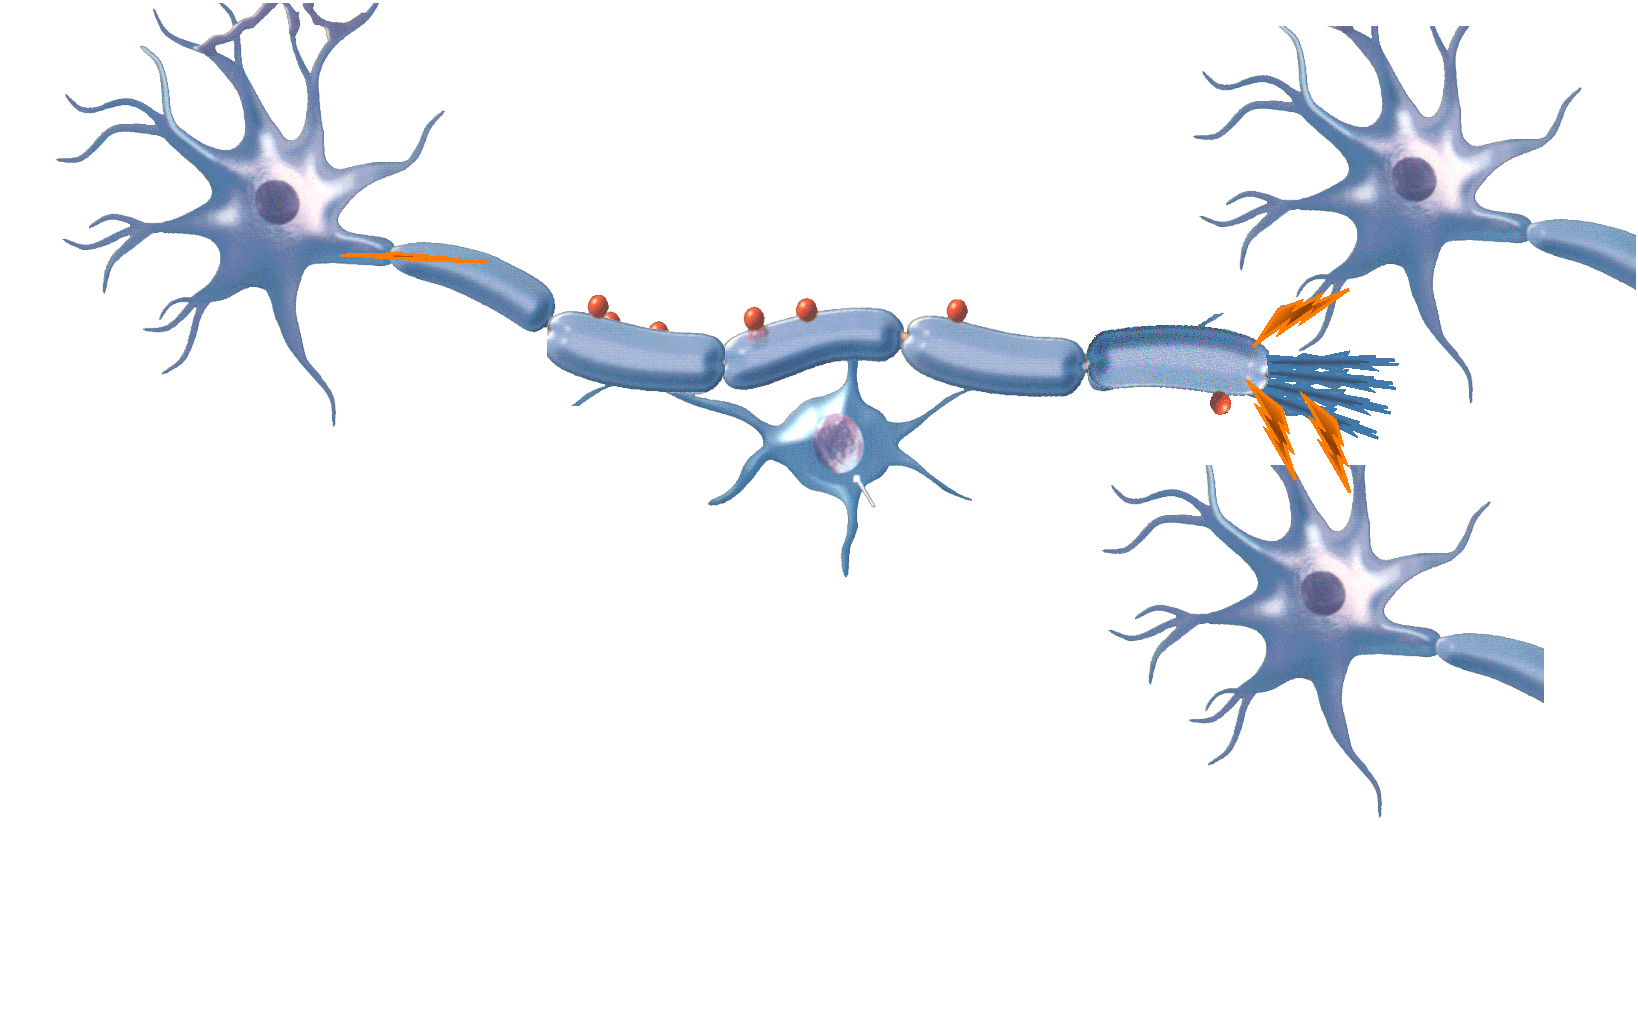
\includegraphics[width=0.5\textwidth]{figures/healthyneuron}};
\node[,below=-1.5cm of healthy] (damaged)
{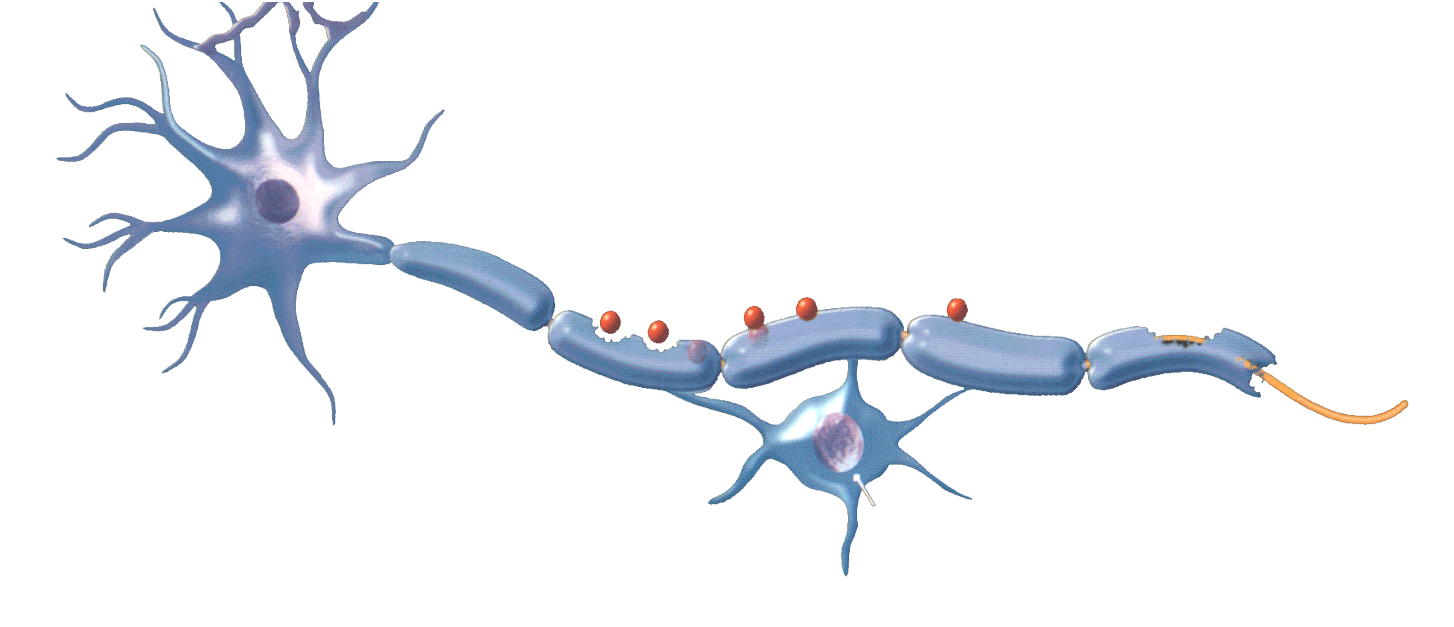
\includegraphics[width=0.5\textwidth]{figures/damagedneuron}};

\node[fit=(healthy)(damaged), inner sep=0] (neurons) {};

\node[right=1cm of neurons] (brain)
{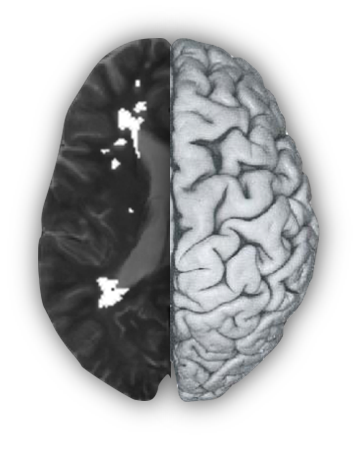
\includegraphics[width=0.4\textwidth]{figures/brain}};

\coordinate (m1) at (-0.75,0.9);
\coordinate (m2) at (0.95,0.9);
\coordinate (m3) at (2.4,-3);

\node[fit=(m1)(m2)] (myelin) {};

\node[above=0.65cm of myelin] (sheaths) {Myelin sheaths};

\draw (m1)--(sheaths);
\draw (m2)--(sheaths);

\node[ellipse,draw=red,thick,minimum width=1.5cm, minimum height=0.9cm,
label=90:Damaged myelin] at (m3) {};

\coordinate (wm) at (7.2,-0.5);
\coordinate (wml) at (6.9,-2.6);

%\draw[red] (wm) circle (3pt);
%\draw[red] (wml) circle (3pt);

\draw[gray,thick] (wm)--(healthy);
\draw[gray,thick] (wml)--(damaged);

%\draw[step=1cm,gray,very thin] (-5,2) grid (10,-6);

\end{tikzpicture}

\caption[Demyelination in MS]{Due to the break down of the blood brain barrier,
the bodies own immune system attacks the myelin sheaths of the axons, which
causes the formation of demyelinating lesions, visible primarily in the white
matter on conventional \gls{mri} scans. Lesions are highlighted in white.}
\end{figure}
 
The clinical presentation of MS is very heterogeneous due to the wide range of
areas of the brain and spinal chord that can be affected. Characteristic but not
specific physical signs and symptoms include the loss of sensitivity or changes
in sensation such as tingling or numbness, which typically starts in the fingers
and toes, as well as muscle weakness, difficulty in moving, difficulties with
coordination and balance, problems with speech or swallowing, visual problems,
feeling tired, acute or chronic pain, and bladder and bowel difficulties. MS can
also lead to cognitive problems such as having difficulties thinking, or
psychiatric and emotional problems such as depression or frequent mood swings.

The course of the disease is unpredictable. However, most patients (around
\SI{80}{\percent}) are initially diagnosed as having \gls{rrms}, which is
characterized by alternating periods of worsening due to inflammatory attacks
and the formation of new lesions, and periods of remission and recovery. The
majority (around \SI{65}{\percent}) of RRMS patients transition to \gls{spms}.
In this stage, the body is no longer able to compensate for the tissue damage,
which leads to the unremitting and progressive accumulation of disability. Other
types of MS include \glslink{ppms}{the primary progressive form (PPMS)},
characterized by the progression of disability from onset with no remissions
after the initial symptoms, and \gls{prms}, which shows progressive accumulation
of disability in addition to clear superimposed relapses.

% TODO: Back this one up with references

\subsection[Measuring disease state and progression]{Measuring Disease State and
Progression}

There is currently no cure for MS. Existing therapies that focus on symptomatic
management and prevention of further damage have variable degrees of
effectiveness, although several recent breakthroughs are promising. To monitor
and further our understanding of the disease, many biomarkers have been
developed that allow for the objective measurement of normal and pathogenic
processes, as well as of the pharmacological response to a therapeutical
intervention \citep{katsavos2013}. The focus of this thesis is on the accurate
measurement of existing imaging biomarkers and the development of new biomarkers
that capture changes in brain morphology and white matter lesions---two
hallmarks of MS pathology. Axonal loss and neurodegeneration can lead to severe
global and regional atrophy. Accurate segmentation of the brain and spinal chord
into its basic tissue types---\gls{csf}, white matter, and gray matter---is a
crucial pre-processing step for deriving imaging biomarkers like brain volume
fraction, cortical thickness, and spinal chord atrophy. In addition, accurate
delineation of lesions is important for measuring lesion count and lesion
volume, two biomarkers that have established their importance for measuring
disease progression and treatment effect.

Many algorithms have been proposed for the accurate and robust segmentation of
the entire brain (BET, ROBEX and the likes) that perform well enough to be used
in routine clinical practice. In contrast, accurate segmentation of lesions has
shown to be a very challenging due to the large variability in lesion size,
shape, intensity, and locations, as well as the large variability in imaging
contrasts produced by scanners used at different clinical sites. Despite a
growing interest in developing fully automatic lesion segmentation methods,
semi-automatic methods are still the standard in routine clinical practice,
although their use is time-consuming, laborious, and potentially biasing. It is
therefore highly desirable to develop a fully-automatic lesion segmentation
method that is robust to large variability, while still being able to segment
lesions with high accuracy and sensitivity.

%
% - biomarkers based on the accurate delineation of lesions such as lesion count
%   and lesion volume
% - To measure those changes accurately, accurate segmentations of different
%   tissue types and lesions are required.
% - A lot of progress has been made to accurately separate the brain from
%   non-brain tissues (brain extraction) and segmenting the brain into its three
%   main tissue types, CSF, WM, GM.
% - Segmenting lesions very challenging due to the large variability in lesion
%   size, shape, contrast, and location as well the the large variability in
%   normal tissue contrasts produced by different scanners at different clinical
%   cites.
% - There is still no fully automatic and robust method for the segmentation of
%   lesions that is robust and accurate enough to be used in routine clinical
%   practice.

Imaging biomarkers used in clinical trials mostly focus on volumetric measures
of global and local changes, which are important and relatively easy to compute,
but only correlate modestly with clinical scores. One reason for the modest
correlation is that they do not reflect potentially important structural
variations, such as shape changes in the brain and the spatial dispersion of
lesions. Therefore, it would be highly desirable to develop biomarkers that
capture potentially important patterns of the variability in brain morphology
and lesion distribution, which would advance our understanding of the complex
pathology of MS.

% TODO: Most of these points should go into the discussion section of why the
% correlations are still not as high as we would wish for.
%
% they only correlate modestly with clinical
% disability scores, which limits their utility for the purpose of personalized
% medicine. There are a number of key reasons why the current imaging biomarkers
% do not have stronger quantitative relationships with clinical scores:
% \begin{itemize}
% 
% \item Due to the wide range of symptoms, MS disability is difficult to score
% comprehensively in routine clinical practice. For example, the Kurtzke expanded
% disability status scale (EDSS)~\citep{Kurtzke:1983} is the most commonly used
% clinical score, but does not account for cognitive impairment, which is a
% significant contributor to disability in the majority of MS
% patients~\citep{Chiaravalloti:2008}.
% 
% \item Through neuroplasticity, the brain and spinal cord can adapt to damage in
% order to maintain functionality~\citep{Tomassini:2012}. As a result, clinically
% silent or subtle pathology is often present.
% 
% \item Conventional MRI does not capture all aspects of MS pathology. For
% example, white matter that appears normal on conventional MRI may actually have
% reduced myelin~\citep{Laule:2004}, a nerve insulator that is critical for proper
% signal conduction. Demyelination is a key pathological feature of MS.
% 
% \item The current established imaging biomarkers largely capture volumetric
% changes, which are important and relatively easy to compute, but do not reflect
% potentially important structural variations, such as shape changes in the brain
% and spatial dispersion of the lesions.
% 
% \end{itemize}
% It would be highly desirable to develop biomarkers that capture potentially
% important patterns of variability in brain morphology and lesion distribution,
% which would advance our understanding of the complex pathology of MS.

% An alternative to using biomarkers for monitoring MS is the use of clinical
% scores. In contrast to biomarkers, clinical scores measure the impact of the
% disease on the patient's life directly through clinical tests. The two most
% widely used scores of measuring disability in MS are the expanded disability
% status scale (EDSS) and the multiple sclerosis function composite. The EDSS
% provides a discrete scale of impairment to ambulation and ranges from 0 (normal
% neurological exam) to 10 (death due to MS). Despite its wide use in clinical
% trials, EDSS have been criticized for putting too much emphasise on the motor
% function of the patient, while ignoring other areas of the patient's life such
% as cognitive functions and upper body movement. The MSFC is a composite score
% composed of the following three subscores: 1) The timed 25 feet walk (T25W)
% measures impairment of the lower limbs, 2) the 9-hole peg test (9-HPT) measures
% impairment of the upper limbs, and 3) the paced auditory serial addition test
% (PASAT) measures impairment of the cognitive function of a patient.
% 
% - Scores don't correlate well with biomarkers
% - Why is this so?
% - Need better biomarkers
% - Maybe introduce clinical scores first then say biomarkers can be used as well
% - Difficulties measuring them
% - Difficulties with correlation to clinical scores

\section[Proposed method]{Proposed Method}

\subsection{Objectives}

% More general and taylored to the challenges. Robust method is the objective.
% Contribution is the development of a method based on neural networks and the
% contributions in there.

The global objective of the thesis is to develop methods that facilitate the
automatic measurement of disease progression and treatment effect. To that end,
we aim to develop a fully automatic lesion segmentation method that is able
to segment lesions accurately under a large range of lesion sizes and in the
presence of varying imaging contrasts and imaging artifacts produced by
different scanners. A second objective was the development of a method that
automatically discovers potentially important patterns of variability in brain
morphology and lesion distribution, with the goal to derive new imaging
biomarkers that correlate stronger with the clinical presentation of the disease
than traditionally used volumetric measures.

\subsection{Overview}

The two methods developed for segmenting MS lesions and recognizing patterns of
variability are both based on algorithms and models that belong to the class of
deep learning approaches. Deep learning is a field within machine learning that
is inspired by the learning capabilities of the brain. Research on the visual
cortex of cats suggests that the receptive fields of neurons are learned from a
continuous stream of images early in the development of the visual system
\citep{wiesel1963}, and fine-tuned later \citep{karni1991}. This allows the
neurons of the visual cortex to adapt to the objects we are working with every
day. While it is difficult, for example, for an average person to recognize the
differences between cows, the feature detecting neurons of the visual system of
cattle farmers are highly tuned to their appearance, allowing them to recognize
individual cows easily. This suggests that a learning based model for
classification should not only learn to perform the requested task based on a
set of pre-defined features, but also learn the features that are most
suitable to perform the task. This kind of end-to-end learning is possible
through the use of deep learning methods, which use multiple layers of nonlinear
processing units to learn a feature hierarchy directly from the input data
without a dedicated feature extraction step.

Deep learning has been successfully used in many research areas such as image
recognition \citep{krizhevsky2012}, speech recognition \citep{hinton2012deep},
natural language understanding \citep{collobert2011natural}, and language
translation \citep{sutskever2014sequence}. Deep learning methods are
particularly successful due to their ability to recognize complex and highly
nonlinear patterns in large amounts of training data, which facilitates the
learning of models that are robust to large variability. This motivates the use
of deep learning methods for segmenting MS lesions, because the large
variability in lesion shape, size, contrast, and location as well as the changes
in imaging contrasts produced by different \gls{mri} scanners make lesion
segmentation a very challenging problem. Furthermore, deep learning cannot only
be used to learn models that are robust to a large range of nonlinear changes,
it can also be used to discover patterns of variability in order to model
complex, recurring and nonlinear changes. This allows deep learning models such
as deep belief networks to be used for manifold learning, e.g., of hand written
digits \citep{hinton2006b} or, as we will show in \ref{sec:manifold}, medical
images \citep{brosch2013}. However, deep learning methods and frameworks were
originally developed for small 2D images and do not scale well to large 3D
images in terms of training time and memory requirements, which prevents the use
of out-of-the-box implementations of deep learning methods for 3D image
analysis.

\subsection{Contributions}

In the course of developing deep learning-based methods for MS lesion
segmentation and pattern discovery, we have made the following main
contributions:
\begin{itemize}
\item We have developed a novel training algorithm for convolutional deep belief
networks and convolutional neural networks that performs training in the
frequency domain. The speed-ups gained by our method compared to spatial domain
implementations and the reduced memory requirements compared to other frequency
domain methods facilitate the application of deep learning to high-resolution
3D medical images.
  
\item We have developed a neural network architecture that jointly learns the
features required to segment MS lesions and to perform the segmentation based on
the automatically learned features. The joint learning of feature extractor and
classifier facilitates the learning of features that are robust to the
variability of MS lesions and varying contrasts produced by different scanners.

\item We have developed a novel objective function for training neural networks
that is suitable for the classification of vastly unbalanced classes, such as
the segmentation of MS lesions, which typically comprise less than one percent
of the image.

\item We have demonstrated that the use of shortcut connections in the proposed
neural network architecture allows for the learning of features at different
scales, which facilitates the segmentation of both very small and very large
lesions.

\item We have developed a framework for modelling changes in brain morphology
and lesion distribution with only a few parameters, which also show improved
correlation with clinical scores compared to established volumetric imaging
biomarkers. In contrast to previous manifold learning approaches, our method
does not assume that the ambient space is locally linear and also does not
require the definition of a suitable similarity measure, or building a proximity
graph.
\end{itemize}

\section[Thesis outline]{Thesis Outline}

The rest of this thesis is subdivided into five chapters as outlined below:

\subsection*{\ref{sec:background}---\nameref{sec:background}}

In this chapter, we will briefly introduce the supervised and unsupervised deep
learning models that form the basis for the lesion segmentation and manifold
learning methods, which are discussed further in \ref{sec:segmentation}
and \ref{sec:manifold}. We will start with a description of dense neural
networks \citep{farley1954,werbos1974,rumelhart1986} and convolutional
neural networks \citep{fukushima1980,lecun1989,lecun1998}. In the second
part, we will give a brief overview of restricted Boltzmann Machines
\citep{freund1992,hinton2010a}, which are the building blocks of deep belief
networks \citep{hinton2006b}.

\subsection*{\ref{sec:training}---\nameref{sec:training}}

Deep learning has traditionally been computationally expensive and advances in
training methods have been the prerequisite for improving its efficiency in
order to expand its application to a variety of image classification problems.
In this chapter, we address the problem of efficient training of convolutional
deep belief networks by learning the weights in the frequency domain, which
eliminates the time-consuming calculation of convolutions. An essential
consideration in the design of the algorithm is to minimize the number of
transformations to and from frequency space. We have evaluated the running time
improvements using two standard benchmark data sets, showing a speed-up of up to
8 times on 2D images and up to 200 times on 3D volumes. In addition, we have
directly compared the time required to calculate convolutions using our method
with the \gls{cudnn}, the current state-of-the-art library for calculating 2D
and 3D convolutions, with the results showing that our method can calculate
convolutions up to 20 times faster than cuDNN. Our training algorithm makes
training of convolutional deep belief networks and convolutional neural networks
on 3D medical images with a resolution of up to \num{128x128x128} voxels
practical, which opens new directions for using deep learning for medical image
analysis.

\subsection*{\ref{sec:segmentation}---\nameref{sec:segmentation}}

In this chapter, we present a novel segmentation approach based on deep 3D
convolutional encoder networks with shortcut connections and apply it to the
segmentation of MS lesions in magnetic resonance images. Our model is a neural
network that consists of two interconnected pathways, a convolutional pathway,
which learns increasingly more abstract and higher-level image features, and a
deconvolutional pathway, which predicts the final segmentation at the voxel
level. The joint training of the feature extraction and prediction pathways
allows for the automatic learning of features at different scales that are
optimized for accuracy for any given combination of image types and segmentation
task. In addition, shortcut connections between the two pathways allow high- and
low-level features to be integrated, which enables the segmentation of lesions
across a wide range of sizes. We have evaluated our method on two publicly
available data sets (MICCAI 2008 and ISBI 2015 challenges) with the results
showing that our method performs comparably to the top-ranked state-of-the-art
methods, even when only relatively small data sets are available for training.
In addition, we have compared our method with five freely available and widely
used MS lesion segmentation methods (EMS, LST-LPA, LST-LGA, Lesion-TOADS, and
SLS) on a large data set from an MS clinical trial.
The results show that our method consistently outperforms these other methods
across a wide range of lesion sizes.

\subsection*{\ref{sec:manifold}---\nameref{sec:manifold}}

Manifold learning of medical images plays a potentially important role for
modeling anatomical variability within a population with applications that
include segmentation, registration, and prediction of clinical parameters.
In this chapter, we describe a novel method for learning the manifold of 3D
brain images and for build a statistical model of brain images that can
automatically discover spatial patterns of variability in brain morphology and
lesion distribution. We propose building such a model using a deep belief
network, a layered network whose parameters can be learned from training
images. In contrast to other manifold learning algorithms, this approach does
not require a prebuilt proximity graph, which is particularly advantageous for
modeling lesions, because their sparse and random nature makes defining a
suitable distance measure between lesion images challenging. Our results show
that this model can automatically learn a low-dimensional manifold of brain
volumes that detects modes of variations that correlate to demographic and
disease parameters. Furthermore, our model can automatically discover the
classic patterns of MS pathology, as well as more subtle ones, and that the
parameters computed have strong relationships to MS clinical scores.

\subsection*{\ref{sec:conclusions}---\nameref{sec:conclusions}}

This chapter concludes the thesis with a brief summary of the addressed problems
and presented results. In the second part, some directions for future are given
in the broader context of deep learning for medical imaging. In particular, we
will give suggestions for new medical image analysis applications of deep
learning and how to deal with relatively small data sets using data
augmentation. In addition, we will discuss two potential advancements of neural
networks that we believe will be particularly important for medical
applications.

%   - Use more data, handle variability better, age of large data is perfect for deep learning
%   - No assumptions other than test data should be similarly distributed than training data -> robust and fast
%   - What can we learn from it? Need visualization of what the network is thinking. Probably relearn what the NN is doing similar to how 
%     brain research works: learn from good and bad cases or from deactivating certain parts of the network to infer what it does.
%   - Theory of learning combining neuroscience and computer science

\begin{comment}

Multiple sclerosis (MS) is a chronic, degenerative disease of the brain and
spinal cord. The clinical presentation of MS is very heterogeneous, and the
range and severity of symptoms can vary greatly between patients. The clinical
course of MS is highly unpredictable, but most patients are initially diagnosed
as having relapsing remitting MS (RRMS), which is characterized by inflammatory
attacks separated by variable periods of remission and recovery. The majority of
RRMS patients will eventually transition into the secondary progressive MS
(SPMS) phase, in which there is an unremitting and progressive accumulation of
disability. There is currently no cure for MS. Existing therapies that focus on
symptomatic management and prevention of further damage have variable degrees of
effectiveness, although several recent breakthroughs are promising. MS pathology
originates at the cellular level and many aspects are not well understood, but
there are characteristic (but not specific) signs of tissue damage, the most
recognizable of which are white matter lesions (WMLs) and brain atrophy, or
shrinkage due to degeneration. These signs can be observed on MRI, which has
become a vital tool for non-invasively monitoring MS patients in the clinic and
for advancing the understanding of MS pathology. WML counts and volume and brain
volume have become established imaging biomarkers for MS clinical trials, and
there is promise for their use in routine clinical practice, but they generally
only correlate modestly with clinical disability scores. The weak link between
the image-based measures of MS pathology and disability scores is known as the
``clinico-radiological paradox'' of MS, and results in the low utility of
current imaging biomarkers for the purposes of personalized medicine. There are
a number of key reasons why the current imaging biomarkers do not have stronger
quantitative relationships with clinical scores:

\begin{itemize}

\item Due to the wide range of symptoms, MS disability is difficult to score
comprehensively in routine clinical practice. For example, the Kurtzke expanded
disability status scale (EDSS)~\citep{Kurtzke:1983} is the most commonly used
clinical score, but does not account for cognitive impairment, which is a
significant contributor to disability in the majority of MS
patients~\citep{Chiaravalloti:2008}.

\item Through neuroplasticity, the brain and spinal cord can adapt to damage in
order to maintain functionality~\citep{Tomassini:2012}. As a result, clinically
silent or subtle pathology is often present.

\item Conventional MRI does not capture all aspects of MS pathology. For
example, white matter that appears normal on conventional MRI may actually have
reduced myelin~\citep{Laule:2004}, a nerve insulator that is critical for proper
signal conduction. Demyelination is a key pathological feature of MS.

\item The current established imaging biomarkers largely capture volumetric
changes, which are important and relatively easy to compute, but do not reflect
potentially important structural variations, such as shape changes in the brain
and spatial dispersion of the lesions.

\item Traditional statistical approaches place a strong emphasis on
interpretability, often at the sacrifice of accuracy, and simple prediction
models such as logistic regression are common. The general assumption is that
the data is generated by a known stochastic data model, with the goodness-of-fit
evaluated by residual analysis, but this works well only with a very low number
of variables~\citep{Breiman2001}.

\end{itemize}

% Add to manifold introduction
Changes in brain morphology and white matter lesions are two hallmarks of MS
pathology, but their variability beyond volumetrics is poorly characterized. To
further the understanding of complex MS pathology,

% Add to segmentation introduction
Focal lesions in the brain and spinal cord are one of the hallmarks of MS
pathology, and are primarily visible in the white matter on structural MRIs.
These lesions are observable as hyperintensities on T2w, proton density-weighted
(PDw), or fluid-attenuated inversion recovery (FLAIR) scans, and as
hypointensities, or ``black holes'' on T1w scans. Imaging biomarkers based on
the identification of lesions, such as lesion count and lesion volume, have
established their importance for assessing disease progression and treatment
effect. However, lesions vary greatly in size, shape, intensity and location,
which makes their automatic and accurate segmentation challenging.

% See literature review as a tool, not as a goal. Try to structure the thesis
% without it and put it where it belongs. Maybe restructure later. I needed a part
% of it already for the motivation. I will put a lot in it when I describe the
% methods. An I will put something in there, when I describe the applications.

\end{comment}